\documentclass[UTF8,titlepage]{article}
\usepackage{amsmath,amssymb,amsthm,amsfonts,amscd}
\usepackage{fontspec}
\setmainfont{Times New Roman}
\usepackage{graphicx}
\usepackage{titlesec}
\usepackage{makecell}
\usepackage{longtable}
\usepackage{xcolor}
\usepackage{tcolorbox}
\usepackage{soul}
\usepackage{adjustbox}
\usepackage{tcolorbox}
\usepackage{enumerate}
\usepackage{pdfpages}
\usepackage{float}
\usepackage{colortbl}
\usepackage{tabularx}
\usepackage{multirow}
\usepackage{pgfplots}
\numberwithin{figure}{section}
\usepackage[left=1.25in,right=1.25in,%
top=1in,bottom=1in]{geometry}
\usepackage{color}
\titleformat{\section}
  {\raggedright\LARGE\bfseries}{\thesection}{1em}{}
\title{Answer for Problem Set 1}
\author{Boyuan Zhao}
\begin{document}
\begin{center}
    {\LARGE \textbf{Answer of Problem Set 2}}\\  % 这就是你的标题
    {\normalsize Boyuan Zhao}\\  % 这就是你的名字
    {\small \today}  % 这是日期
\end{center}
\section{Problem 1. Addictive goods.}
\begin{enumerate}
    \item An approximate map of indifference curves:
    \begin{figure}[H]
    \centering
     \resizebox{0.75\textwidth}{!}{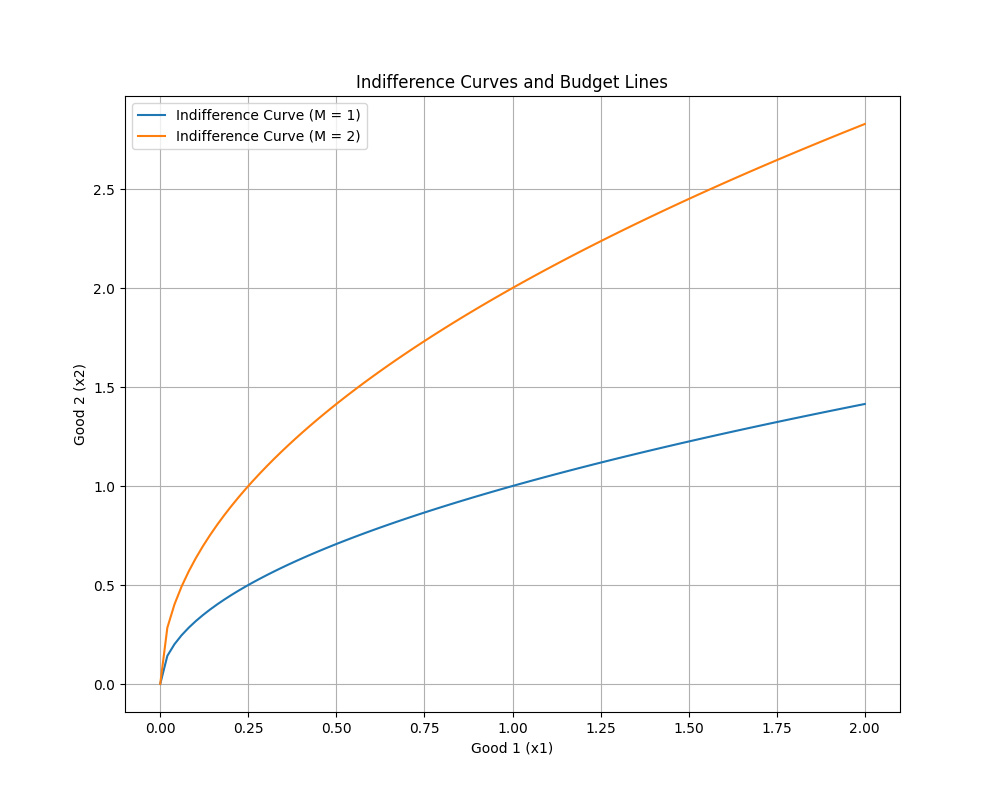
\includegraphics{/workspaces/TexFile/indifference_curves.png}}
     \caption{indifference Curves}
     \label{}
    \end{figure}
    \item The derivative of the utility function with respect to $r_1$ is:
    \[\frac{\partial u}{\partial r_1} = -\alpha(x_1 - r_1)^{\alpha-1} x_2^\beta\]
    This term is negative because as the reference point $r_1$ (i.e., addiction level) increases, the utility from consuming a certain quantity of the addictive good $x_1$ decreases. This is because a higher addiction level reduces the marginal benefit from consuming the good.
    \item The marginal utility with respect to $x_1$ is:
    \[\frac{\partial u}{\partial x_1} = \alpha(x_1 - r_1)^{\alpha-1} x_2^\beta\]
    and the derivative of this marginal utility with respect to $r_1$ is:
    \[\frac{\partial^2 u}{\partial x_1 \partial r_1} = -\alpha(\alpha - 1)(x_1 - r_1)^{\alpha-2} x_2^\beta\]
    This term is positive because the more accustomed a person becomes to the addictive good (i.e., the higher their addiction level $r_1$), the more they will want to consume the addictive good (i.e., the higher the marginal utility of $x_1$).
    \item The Lagrangian for this maximization problem is:
    \[L = (x_1 - r_1)^\alpha x_2^\beta + \lambda(M - p_1x_1 - p_2x_2)\]
    \item The first order conditions for this problem are given by the partial derivatives of the Lagrangian with respect to $x_1$, $x_2$ and $\lambda$:
    \[\frac{\partial L}{\partial x_1} = \alpha(x_1 - r_1)^{\alpha-1} x_2^\beta - \lambda p_1 = 0\]
    \[\frac{\partial L}{\partial x_2} = \beta (x_1 - r_1)^\alpha x_2^{\beta-1} - \lambda p_2 = 0\]
    \[\frac{\partial L}{\partial \lambda} = M - p_1 x_1 - p_2 x_2 = 0\]
    \item Solving these equations gives us the optimal values of $x_1$ and $x_2$:
    \[x^*_1 = \frac{\alpha M + \beta r_1 p_2}{p_1}\]
    \[x^*_2 = \frac{\beta M}{p_2}\]
    \item The minimum level of income such that the solution makes sense (i.e., $x_1^* \geq r_1$ and $x_2^* \geq 0$):
    \[M \geq max(\frac{r_1 p_1}{\alpha}, 0)\]
    \item The derivative of $x_1^*$ with respect to $M$ is:
    \[\frac{dx^*_1}{dM} = \frac{\alpha}{p_1}\]
    This result is always positive, meaning that good $x_1$ is a normal good.
    \item The derivative of $x_1^*$ with respect to $r_1$ is:
    \[\frac{dx^*_1}{dr_1} = \frac{\beta p_2}{p_1}\]
    This result is positive, indicating that as addiction level $r_1$ increases, the quantity of good $x_1$ consumed increases. This makes sense because a higher addiction level increases the desire to consume the addictive good.
    \item The derivative of $x_2^*$ with respect to $r_1$ is zero, indicating that the quantity of good $x_2$ consumed does not depend on the addiction level $r_1$. This result is consistent with the idea that drug addicts can spend virtually all of their income on drugs and none on other goods.
    \item Using the envelope theorem, the derivative of the optimal utility with respect to $r_1$ is:
    \[\frac{d}{dr_1} u(x_1^*(p_1, p_2, M, r_1), x_2^*(p_1, p_2, M, r_1), r_1) = -\alpha(x_1^* - r_1)^{\alpha-1} x_2^{\beta}\]
    This indicates that as the addiction level increases, the utility at the optimum decreases, reflecting the decreased satisfaction from consuming the addictive good as addiction grows.
\end{enumerate}
\clearpage
\section{Problem 2. Quasi-linear preferences.}
\begin{enumerate}
  \item The Lagrangian for this maximization problem is:
  \[L = \phi(x_1) + x_2 + \lambda(M - p_1x_1 - p_2x_2)\]
  \item The first order conditions for this problem are given by the partial derivatives of the Lagrangian with respect to $x_1$, $x_2$ and $\lambda$:
  \[\frac{\partial L}{\partial x_1} = \phi'(x_1) - \lambda p_1 = 0\]
  \[\frac{\partial L}{\partial x_2} = 1 - \lambda p_2 = 0\]
  \[\frac{\partial L}{\partial \lambda} = M - p_1 x_1 - p_2 x_2 = 0\]
  \item From the first order condition for $x_2$, we see that $\lambda = 1/p_2$. This implies that $\lambda$ does not depend on $p_1$ or $M$, which usually isn't the case. In this context, $\lambda$ can be interpreted as the marginal utility of wealth. Because the utility function is linear in $x_2$, the marginal utility of $x_2$ (which equals 1) is constant, so the marginal utility of wealth is also constant.
  \item Plugging the value of $\lambda$ into the first order condition for $x_1$, we get:
  \[\phi'(x_1) = \frac{p_1}{p_2}\]
  This equation implicitly defines $x_1^*$ as a function of the parameters $p_1$, $p_2$, $M$. However, we see that $x_1^*$ does not depend on income $M$, which means that good 1 is a neutral good.
  \item From the first order condition with respect to $x_1$, taking derivative with respect to $p_1$, we obtain:
  \[\frac{d x_1^*}{dp_1} = -\frac{\phi''(x_1^*)}{\phi''(x_1^*)} < 0\]
  This is consistent with our expectation that an increase in the price of a good will decrease its demand (holding everything else constant). The demand for good 1 is solely determined by its own price and does not depend on income.
  \item When $u(x_1, x_2) = {x_1}^{\frac{1}{2}} + x_2$, the first order conditions become:
  \[\frac{1}{2\sqrt{x_1}} = \frac{p_1}{p_2}\]
  \[1 = \frac{1}{p_2}\]
  Solving these equations, we find:
  \[x_1^* = \frac{p_1^2}{4}\]
  \[x_2^* = M - p_1 x_1^*\]
  \item $x_2^*$ will be nonnegative as long as $M \geq p_1 x_1^*$, i.e., as long as income is at least as large as the expenditure on good 1.
  \item The equation of the indifference curve is given by $x_2 = u - \sqrt{x_1}$. For simplicity, let's consider several different values for utility u, say u = 1, 2, 3.
  
  The indifference curves can be graphically represented as follows:

  \begin{figure}[H]
  \centering
   \resizebox{0.75\textwidth}{!}{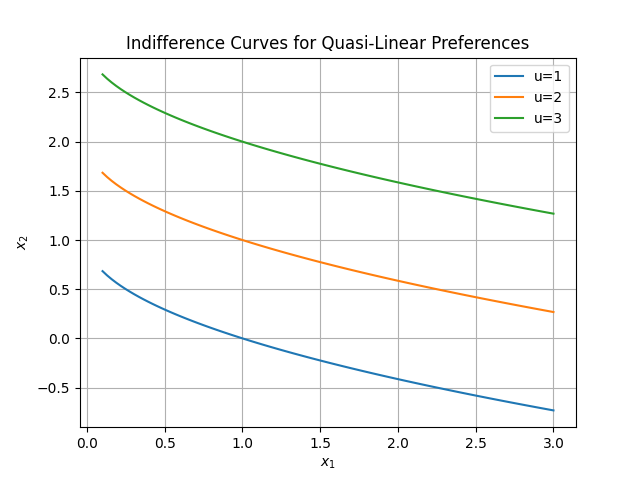
\includegraphics{/workspaces/TexFile/Microeconomic/graph/q8.png}}
   \caption{The indifference curves}
   \label{}
  \end{figure}

  In this graph, the x-axis represents $x_1$ and the y-axis represents $x_2$. Different curves represent different levels of utility u. As you can see, the curves are vertical lines for $x_1=0$ and flatten as $x_1$ increases.

This shape of indifference curves is quite unique and contrasts with the more conventional Cobb-Douglas preferences. For Cobb-Douglas preferences, the indifference curves are downward sloping and convex to the origin, indicating a constant rate of trade-off between $x_1$ and $x_2$. The marginal rate of substitution between the two goods is not constant but depends on the quantities of both goods.

On the contrary, with these quasi-linear preferences, the marginal rate of substitution is constant and does not depend on the quantity of good 1 consumed. This is shown by the straight line of the indifference curve. The consumer is willing to give up the same amount of $x_2$ for additional $x_1$, regardless of how much $x_1$ they are already consuming. This reflects a constant marginal utility of $x_1$.

Also, there is no satiety point - a point beyond which consuming more of $x_1$ doesn't increase utility, which is a usual case in many utility functions. Here, the consumer will keep increasing the consumption of $x_1$ as long as they have more money to spend, as the utility increases with $x_1$.
  \item The graph is shown below:
  \begin{figure}[H]
  \centering
   \resizebox{0.75\textwidth}{!}{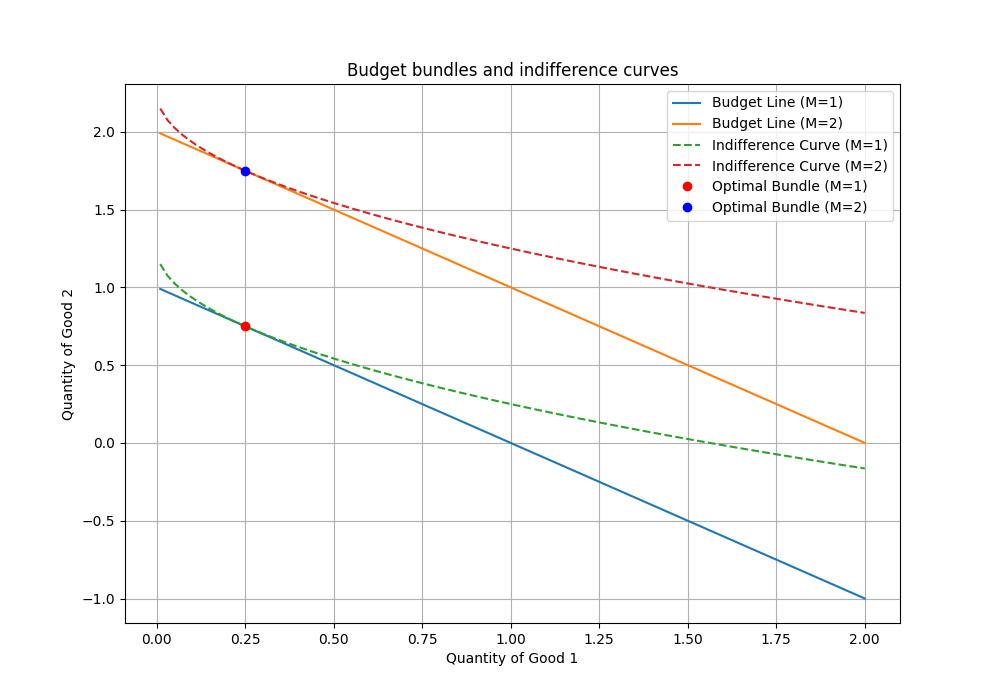
\includegraphics{/workspaces/TexFile/Microeconomic/graph/q9.png}}
   \caption{Budget bundles and indifference curves}
   \label{}
  \end{figure}

  For the given budget lines, the optimal consumption bundles are found by equating the marginal rate of substitution (which is constant at $p_1/p_2$) to the slope of the budget line. The bundle is at the point where the indifference curve is tangent to the budget line. Since the price ratios are the same in both cases, the optimal quantity of good 1 is the same. The increase in income goes entirely toward good 2, confirming the absence of an income effect for good 1.

\end{enumerate}
\end{document}